%!TEX root = thesis.tex
\documentclass[
11pt,
a4paper,
abstracton,
numbers=noenddot,
listof=totoc,
bibliography=totoc,
openright,
cleardoublepage=plain,
parskip=half+, % comment this out if you do not want an empty half line between paragraphs, but please read the KomaScript Guide and search for parskip (around page 82): ftp://ftp.dante.de/pub/tex/macros/latex/contrib/koma-script/scrguide.pdf
BCOR=1cm, % Bindekorrektur: Change this accordingly, also read the KomaScript Guide! Make sure you read the guide.
]{scrreprt}

% % % % % % % % % % % % % % % % % % % % % % % % % % % % % % % % %
% EDIT THE DATA IN THIS BLOCK TO YOUR INFORMATION				%
% % % % % % % % % % % % % % % % % % % % % % % % % % % % % % % % %
% Set data about yourself										%
\newcommand{\authorname}{Jan Philipp Berg, Simon Keil}								%
\newcommand{\studentnumber}{000000}	% Matrikelnummer			%
\newcommand{\courseofstudy}{Information Systems} % Studiengang	%
																%
% Set data about your thesis									%
\newcommand{\thesistitle}{Implementation of the Advanced Encryption Standard - Documentation}		%
\day=04 \month=02 \year=2021									%
																%
% Set thesis type and language									%
\newcommand{\thtype}{Seminar}	% Bachelor, Master or Seminar	%
\newcommand{\thesislanguage}{English}	% English or German		%
% % % % % % % % % % % % % % % % % % % % % % % % % % % % % % % % %

% if you really need additionall packages include them here
%\usepackage{package}


% DO NOT EDIT THE _settins FILE!
% General stuff
\usepackage{fixltx2e}
\usepackage[utf8]{inputenc} % CHANGE HERE IF NECESSARY
\usepackage[T1]{fontenc}
\usepackage[english]{babel} % last language given is used (here: english) #ngerman,
%\usepackage{microtype}
\usepackage{ifpdf}
\usepackage{verbatim}
\usepackage{float}

\author{\authorname}
\title{\thesistitle}
\date{\today}

% Figures
\usepackage{graphicx}
\usepackage{subfig}
\usepackage{placeins}

% Tables
\usepackage{booktabs}
\usepackage{marvosym}
\usepackage{multirow}

% Math stuff and units
\usepackage{latexsym,amsmath, amssymb, amsfonts, upgreek}
\usepackage{siunitx}
\newcommand{\mathup}{\mathrm}

% Acronyms
\usepackage[printonlyused]{acronym}

% Enable quotes by \enquote{}
\usepackage[babel,english=american]{csquotes}

% Necessary for frontpage, allows to create automata and fancy graphics
\usepackage{tikz}

% Protocols and bytefields
\usepackage{protocol}
\usepackage{bytefield}

% Source code listings
\definecolor{colKeys}{rgb}{0,0,1}
\definecolor{colIdentifier}{rgb}{0,0,0}
\definecolor{colComments}{rgb}{1,0,0}
\definecolor{colString}{rgb}{0,0.5,0}

\usepackage{listings}
\lstset{%
	float=hbp,%
	basicstyle=\ttfamily\scriptsize, %
	identifierstyle=\color{colIdentifier}, %
	keywordstyle=\color{colKeys}, %
	stringstyle=\color{colString}, %
	commentstyle=\color{colComments}, %
	columns=flexible, %
	tabsize=2, %
	frame=single, %
	extendedchars=true, %
	showspaces=false, %
	showstringspaces=false, %
	numberstyle=\tiny, %
	breaklines=true, %
	backgroundcolor=, %
	breakautoindent=true, %
	captionpos=b%
}

% Algorithms
\usepackage[ruled, vlined, linesnumbered, algosection, algo2e]{algorithm2e}

% Format page foot and header
\usepackage{scrlayer-scrpage}
\clearscrheadings
\clearscrheadfoot
\automark[section]{chapter}
\ohead{\pagemark}
\ihead{\headmark}
\pagestyle{scrheadings}

%% use some standards for mathematical expressions:
\newcommand{\red}{{\rm red}}
\newtheorem{theorem}{Theorem}[section]
\newtheorem{lemma}[theorem]{Lemma}
\newtheorem{proposition}[theorem]{Proposition}
\newtheorem{corollary}[theorem]{Corollary}
% \newtheorem{definition}[theorem]{Definition}
\newtheorem{algorithm}[theorem]{Algorithm}
\newenvironment{example}{\begin{quote}{\bf Example:}}{\end{quote}}

% Bibliography
\bibliographystyle{alpha}

% gray definition boxes, that whay you'll find them in the text
\usepackage{shadethm}
\newshadetheorem{sthm}{Definition}[chapter]
\newenvironment{definition}[1][]{
	\definecolor{shadethmcolor}{rgb}{.9,.9,.9}
	\begin{sthm}[#1]
	}{\end{sthm}}

% experimental
%\usepackage{scrhack}
\usepackage{paralist}
% Hyperlinks and menu for your document
\usepackage[breaklinks,hyperindex,colorlinks,anchorcolor=black,citecolor=black,filecolor=black,linkcolor=black,menucolor=black,urlcolor=black,pdftex]{hyperref}

% pagebackref: Add page number to the references where they can be found
% DO NOT LOAD ANY OF YOUR PACKAGES BEYOND THIS PACKAGE

\makeatletter
\AtBeginDocument{
	\hypersetup{
		pdftitle = {\@title},
		pdfauthor = {\@author},
		pdfsubject={\@title},
		pdfkeywords={Template, LaTeX, SysSec, Sensor fingerprinting, Accelerometer, Smartphone, Mobile Device}, % CHANGE HERE
		%    unicode={true},
	}
}
\makeatother

% \ifpdf
% 	\hypersetup{linktocpage=false} 	% false=links are section names, true=links are page numbers, IMPORTANT: in dvi2ps mode, 'true' is required!
% \else
% 	\hypersetup{linktocpage=true} 		% false=links are section names, true=links are page numbers, IMPORTANT: in dvi2ps mode, 'true' is required!
%  \usepackage[hyphenbreaks]{breakurl}
% \fi

\newcommand{\declarationofauthorship}[2]{%
	\ifthenelse{\equal{#1}{German}}
	{\chapter*{Eidesstattliche Erklärung}
	Ich versichere hiermit, dass ich diese \thtype-Arbeit mit dem Titel \glqq{#2}\grqq
	selb\-st\"{a}n\-dig und ohne fremde Hilfe angefertigt habe, und dass ich alle von anderen Autoren w\"{o}rtlich \"{u}\-ber\-nom\-men\-en Stellen wie auch die sich an die Ge\-dan\-ken\-g\"{a}n\-ge anderer Autoren eng anlehnenden Aus\-f\"{u}h\-run\-gen meiner Arbeit besonders
	gekennzeichnet und die Quellen zitiert habe.

	\vspace{2cm}
	\rule{4cm}{0.1pt} \hfill \rule{7cm}{0.1pt} \\
	\hspace*{1.75cm} \textsc{Datum} \hspace*{6.8cm} \textsc{Unterschrift}
	}
	{\chapter*{Declaration}
		I hereby declare that, to the best of my knowledge and belief, this \thtype thesis titled ``{#2}'' is my own work. I confirm that each significant contribution to and quotation in this thesis that originates from the work or works of others is indicated by proper use of citation and references.

	\vspace{2cm}
	\rule{4cm}{0.1pt} \hfill \rule{7cm}{0.1pt} \\
	\hspace*{1.75cm} \textsc{Date} \hspace*{6.8cm} \textsc{Signature}
	}
}


\newcommand{\consentforplagiarismdetection}[5]{%
	\ifthenelse{\equal{#1}{German}}
	{\chapter*{Einverständniserklärung}
		{\small
		zur Prüfung meiner Arbeit mit einer Software zur Erkennung von Plagiaten

		\begingroup
			\textbf{Name}:~{#2}\newline
			\textbf{Matrikelnummer}:~{#3}\newline
			\textbf{Studiengang}:~{#4}\newline
			\textbf{Titel der Arbeit}:~{#5}\newline
		\endgroup

		\textbf{Was ist ein Plagiat?}
		Als ein Plagiat wird eine Übernahme fremden Gedankengutes in die eigene Arbeit angesehen, bei der die Quelle, aus der die Übernahme erfolgt, nicht kenntlich gemacht wird. Es ist dabei unerheblich, ob z.B. fremde Texte wörtlich übernommen werden, nur Strukturen (z.B. argumentative Figuren oder Gliederungen) aus fremden Quellen entlehnt oder Texte aus einer Fremdsprache übersetzt werden.

		\textbf{Softwarebasierte Überprüfung}
		Alle Bachelor- und Masterarbeiten werden vom Prüfungsamt mit Hilfe einer entsprechenden Software auf Plagiate geprüft. Die Arbeit wird zum Zweck der Plagiatsüberprüfung an einen Software-Dienstleister übermittelt und dort auf Übereinstimmung mit anderen Quellen geprüft. Zum Zweck eines zukünftigen Abgleichs mit anderen Arbeiten wird die Arbeit dauerhaft in einer Datenbank gespeichert. Ein Abruf der Arbeit ist ausschließlich durch die Wirtschaftswissenschaftliche Fakultät der Westfälischen Wilhelms-Universität Münster möglich. Der Studierende erklärt sich damit einverstanden, dass allein zum beschriebenen Zweck der Plagiatsprüfung die Arbeit dauerhaft gespeichert und vervielfältigt werden darf. Das Ergebnis der elektronischen Plagiatsprüfung wird dem Erstgutachter mitgeteilt.

		\textbf{Sanktionen}
		Liegt ein Plagiat vor, ist dies ein Täuschungsversuch i.S. der Prüfungsordnung, durch den die Prüfungsleistung als \enquote{nicht bestanden} gewertet wird. Es erfolgt eine Mitteilung an das Prüfungsamt und die dortige Dokumentation. In schwerwiegenden Täuschungsfällen kann der Prüfling von der Prüfung insgesamt ausgeschlossen werden. Dies kann unter Umständen die Exmatrikulation bedeuten. Plagiate können auch nach Abschluss des Prüfungsverfahrens und Verleihung des Hochschulgrades zum Entzug des erworbenen Grades führen.


		Hiermit erkläre ich, dass ich die obigen Ausführungen gelesen habe und mit dem Verfahren zur Aufdeckung und Sanktionierung von Plagiaten einverstanden bin.
		}

		\vspace{2cm}
		\rule{4cm}{0.1pt} \hfill \rule{7cm}{0.1pt} \\
		\hspace*{1.75cm} \textsc{Datum} \hspace*{6.8cm} \textsc{Unterschrift}
	}
	{\chapter*{Consent Form}
	{\small
		for the use of plagiarism detection software to check my thesis

		\begingroup
		\textbf{Full Name}:~{#2}\newline
		\textbf{Student Number}:~{#3}\newline
		\textbf{Course of Study}:~{#4}\newline
		\textbf{Title of Thesis}:~{#5}\newline
		\endgroup

		\textbf{What is plagiarism?}
		Plagiarism is defined as submitting someone else's work or ideas as your own without a complete indication of the source. It is hereby irrelevant whether the work of others is copied word by word without acknowledgment of the source, text structures (e.g. line of argumentation or outline) are borrowed or texts are translated from a foreign language.

		\textbf{Use of plagiarism detection software}
		The examination office uses plagiarism software to check each submitted bachelor and master thesis for plagiarism. For that purpose the thesis is electronically forwarded to a software service provider where the software checks for potential matches between the submitted work and work from other sources. For future comparisons with other theses, your thesis will be permanently stored in a database. Only the School of Business and Economics of the University of Münster is allowed to access your stored thesis. The student agrees that his or her thesis may be stored and reproduced only for the purpose of plagiarism assessment. The first examiner of the thesis will be advised on the outcome of the plagiarism assessment.

		\textbf{Sanctions}
		Each case of plagiarism constitutes an attempt to deceive in terms of the examination regulations and will lead to the thesis being graded as \enquote{failed}. This will be communicated to the examination office where your case will be documented. In the event of a serious case of deception the examinee can be generally excluded from any further examination. This can lead to the exmatriculation of the student. Even after completion of the examination procedure and graduation from university, plagiarism can result in a withdrawal of the awarded academic degree.

		I confirm that I have read and understood the information in this document. I agree to the outlined procedure for plagiarism assessment and potential sanctioning.
		}

		\vspace{2cm}
		\rule{4cm}{0.1pt} \hfill \rule{7cm}{0.1pt} \\
		\hspace*{1.75cm} \textsc{Date} \hspace*{6.8cm} \textsc{Signature}
	}
}


% your document starts here
\begin{document}

% title page - no need to edit
% !TEX root = thesis.tex
\begin{titlepage}
\makeatletter

\enlargethispage{3cm}

\begin{minipage}{0.45\textwidth}
	
\includegraphics[width=\textwidth]{data/assets/wwu-logo}
\end{minipage}
%\hfill
\hspace{.1\textwidth}
\begin{minipage}{0.45\textwidth}
	
\includegraphics[width=\textwidth]{data/assets/faculty-de}
\end{minipage}


\vspace*{10cm}
\begin{minipage}[b]{1\linewidth}
	\sffamily
  	\hspace{-17.2mm}
  	% \includegraphics[scale=1.0]{data/logo/rub_slogan}\\

   	\textbf{\LARGE {\@title}}\\

  	\Large{\@author}\\

% 	\vspace*{35mm}
	\vspace{4cm}
  	\normalsize{
   	\thtype\/ Thesis\@~~--~~\@date\@.\\
   	Cyber Security\\Department of Information Systems\\
   	University Münster, Germany\\}
	\newline
	\normalsize{
	\begin{tabular}{@{}ll@{}}
	Principal Supervisor: Prof.~Dr.-Ing.~Thomas~Hupperich\\
%	Associate Supervisor: XXXXXXXXXX\\
	%Advisor: & Another Guy, Maybe Another\\
	\end{tabular}
	}
\end{minipage}


\makeatother
\end{titlepage}


% give a short abstract of your thesis


\cleardoublepage
\pagestyle{scrheadings} % reenable headers and footers
\tableofcontents

% include all your chapters as .tex files,
% each file contains sections \section{name of section},
% subsections \subsections{...} and so on...

\chapter{Introduction} \label{chap:intro}
%\pagenumbering{arabic} %switches to arabic numbers for the rest of the text

%!TEX root = thesis.tex
\chapter{Quickstart Guide}

This program implements several modes of the AES-128 algorithm to encrypt and decrypt data. This section details the requirements and installation process, as well as the execution of those modes.

\section{Installation}

The program is written in C and Python3. It requires a current python interpreter as well as a compiler for the parts written in C. The requirements are:
\begin{itemize}
  \item Python 3.6 or newer (with the pip/pip3 installed)
  \item a current version of gcc/clang (has to be on PATH as well)
  \item a Unix-Like operating system
\end{itemize}

If the above requirements are met, copy the program to the desired location. Optionally you could use \lstinline{pyenv} or \lstinline{virtualenv} to create a virtual python environment to run in. In order to install the python dependencies run:
\begin{lstlisting}
  pip3 install -r requirements.txt
\end{lstlisting}

When the python dependencies are installed simply run the \lstinline{aes} script. On the first execution it will try to compile the .C files into shared-object libraries. The program is now fully setup and ready to use.

\section{Usage Guide}
The program has four main commands and corresponding modes of operation:
\begin{itemize}
  \item text encrypt -  \lstinline{te}
  \item text decrypt -  \lstinline{td}
  \item file encrypt -  \lstinline{fe}
  \item file decrypt -  \lstinline{fd}
\end{itemize}
To get help on the program itself or each command specifically run \lstinline{./aes [COMMAND] --help}.

\subsection{Text Encrypt}
The command \lstinline{te} makes the program encrypt a text given on the command line. The command is structured as follows:
\begin{lstlisting}
  aes te [OPTIONS] PASSWORD CIPHERTEXT

  Options:
  -k, --key  use 16-byte hexadecimal key instead of password of arbitrary length
  -h, --hex  interpret the input as pure unencoded hexadecimal bytes
\end{lstlisting}

The \lstinline{PASSWORD} argument takes a string of arbitrary length and creates a key out of it. If you want to give an explicit AES-128 16 byte key, use the \lstinline{-k/--key} option. The \lstinline{CIPHERTEXT} argument takes the text to be encrypted. By default it is interpreted as \lstinline{UTF-8}. If you want to explicitly give raw hexadecimal input, use the \lstinline{-h/--hex} option.

Usage of the command with password \enquote{correcthorsebatterystaple} and text \enquote{https://xkcd.com/936/} would look like this:
\begin{lstlisting}
> ./aes te correcthorsebatterystaple "https://xkcd.com/936/"
495bdfc4470ba9b320d1dffcc6b58f762fa21f4624d846803d08f3e236dac08b
\end{lstlisting}

Encryption of the same text with an explicit hexadecimal key would look like this:
\begin{lstlisting}
> ./aes te --key 0000ffff0000ffff0000ffff0000ffff "https://xkcd.com/936/"
690beeaa673a942e5035d2f771a7c5683e8bd069afc4b3d5f5201d4f90f30a37
\end{lstlisting}

Encryption of a sample block from the FIPS 197 AES standard document \cite{aes2001} would look like this:
\begin{lstlisting}
> ./aes te --key 000102030405060708090a0b0c0d0e0f --hex 00112233445566778899aabbccddeeff
69c4e0d86a7b0430d8cdb78070b4c55a
\end{lstlisting}

\subsection{Text Decrypt}
The command \lstinline{td} makes the program decrypt a ciphertext given on the command line. The command is structured as follows:
\begin{lstlisting}
  aes td [OPTIONS] PASSWORD CIPHERTEXT

Options:
  -k, --key  use 16-byte hexadecimal key instead of password of arbitrary length
  -h, --hex  output raw hexadecimal without encoding
\end{lstlisting}
The \lstinline{PASSWORD} argument takes a string of arbitrary length and creates a key out of it. If you want to give an explicit AES-128 16 byte key, use the \lstinline{-k/--key} option. \lstinline{CIPHERTEXT} argument takes the text to be decrypted. By default the output will be decoded \lstinline{UTF-8}. If you want to see the raw hex ouput instead, or if you expect the output to not be \lstinline{UTF-8} decodable, use the \lstinline{-h/--hex} option.

Usage of the command with password \enquote{correcthorsebatterystaple} and an encrypted text would look like this:
\begin{lstlisting}
> ./aes td correcthorsebatterystaple
>      495bdfc4470ba9b320d1dffcc6b58f762fa21f4624d846803d08f3e236dac08b
https://xkcd.com/936/
\end{lstlisting}

Decryption of the sample block from FIPS 197 \cite{aes2001} has the following input and output:
\begin{lstlisting}
> ./aes td --key 000102030405060708090a0b0c0d0e0f --hex 69c4e0d86a7b0430d8cdb78070b4c55a
00112233445566778899aabbccddeeff
\end{lstlisting}


\subsection{File Encrypt}
The command \lstinline{fe} makes the program encrypt a given file with AES-128. The command is structured as follows:
\begin{lstlisting}
aes fe [OPTIONS] PASSWORD FILEPATH_IN [CHUNKSIZE]

Options:
  -k, --key  use 16-byte hexadecimal key instead of password of arbitrary length
\end{lstlisting}
The \lstinline{PASSWORD} argument takes a string of arbitrary length and creates a key out of it. If you want to give an explicit AES-128 16 byte key, use the \lstinline{-k/--key} option. The \lstinline{FILEPATH_IN} argument takes a relative or absolute path to the file to be encrypted. The output file will have the same name and location as the input file, only with the \enquote{.enc} file extension added. The program processes the file in chunks of size 33554432 bytes (33 MB). Optionally the chunksize can be changed by giving it at the end of the command.

Encryption of the local file \lstinline|foo| with password \lstinline|correcthorsebatterystaple| would look like this:
\begin{lstlisting}
> ./aes fe correcthorsebatterystaple foo
\end{lstlisting}
The output is the file \lstinline|foo.enc|.


\subsection{File Decrypt}
The command \lstinline{fd} makes the program decrypt a given file with AES-128. The command is structured as follows:
\begin{lstlisting}
aes fd [OPTIONS] PASSWORD FILEPATH_IN [CHUNKSIZE]

Options:
-k, --key    use 16-byte hexadecimal key instead of password of arbitrary length
-f, --force  force decryption of files without a .enc file extension.
             Will add a .decrypted extension on the output.
\end{lstlisting}
The \lstinline{PASSWORD} argument takes a string of arbitrary length and creates a key out of it. If you want to give an explicit AES-128 16 byte key, use the \lstinline{-k/--key} option. The \lstinline{FILEPATH_IN} argument takes a relative or absolute path to the file to be decrypted. The command expects a file with the \enquote{.enc} file extension. If you want to decrypt a file without that extension use the \lstinline{-f/--force} option.

Decrypting the local file \lstinline|foo.enc| with password \lstinline|correcthorsebatterystaple| requires the following input:
\begin{lstlisting}
> ./aes fd correcthorsebatterystaple foo.enc
\end{lstlisting}
The output is the file \lstinline|foo|.

Decryption of an encrypted local file \lstinline|bar| with the \enquote{.enc} file extention looks like this:
\begin{lstlisting}
> ./aes fd --force correcthorsebatterystaple bar
\end{lstlisting}
The output will be the file \lstinline|bar.decrypted|.


%!TEX root = thesis.tex
\chapter{Functions - Decryption}
\label{ch:decryption}

AES is a symmetric encryption algorithm. Therefore the decryption is the inverse of the encryption. As AES encryption works on 16 byte blocks, the decryption does the same. There are also the same number of rounds.

\section{Decryption of Multiple Blocks}
\label{ch:dec_multipleblocks}
The \lstinline|decryptBlocks| function is used when an input of more than 16 bytes (one block) has to be decrypted. It assumes a padded input, meaning the input array has to be of a length divisible by 16. Padding is handled in the wrapper and can therefore be taken as a given.

\textbf{Args:}
\begin{itemize}
  \item \lstinline{uint8_t *bytes} a pointer to the data to be decrypted
  \item \lstinline{const uint8_t *keys} a pointer to the key-bytearray
  \item \lstinline{const size_t length} the length of the data array
\end{itemize}

\textbf{Returns:}
\begin{itemize}
  \item The function does not return anything as the work is done on the data that the \lstinline{*bytes} pointer references. It can simply be read out of memory afterwards.
\end{itemize}

\subsection{Order of Operations}
The function simply loops over the data in 16 byte steps and calls the \lstinline{decryptBlock} function on each of the blocks. This mode of operation of encrypting and decrypting multiple blocks each by itself is (as previously mentioned) called \enquote{Electronic Code Book Mode} (\ac{ECB}).

\section{Decrypt Block}
\label{ch:dec_block}
The \lstinline{decryptBlock} function outlines the main part of the AES decryption algorithm. It calls all the functions that do operations on the data in the right order.

\textbf{Args:}
\begin{itemize}
  \item \lstinline{uint8_t *bytes} a pointer to the data to be decrypted
  \item \lstinline{const uint8_t *keys} a pointer to the key-bytearray
\end{itemize}

\textbf{Returns:}
\begin{itemize}
  \item The function does not return anything as the work is done on the data that the \lstinline{*bytes} pointer references. It can simply be read out of memory afterwards.
\end{itemize}

\subsection{Order of Operations}
The function strictly follows the order of the inverse cipher given in the FIPS 197 (Chapter 5.3 Figure 12) standard document. The order is as follows:
\begin{enumerate}
  \item The last round-key is added to the data. As the key-bytearray is passed to the function in reverse order, the first key of the array can be used here. The function that is being called for this step is called \lstinline{addRoundKey}.
  \item A for-loop with nine iterations is initiated.
  \item The \lstinline{inverseShiftRows} function is called to shift the data around in the block.
  \item The \lstinline{inverseSubBytes} function substitutes the values in the block with values from the inverse S-Box.
  \item The next round-key is added.
  \item The columns are mixed via multiplication and addition in the \lstinline{inverseMixColumns} function.
  \item The for-loop closes.
  \item The inverse shift-rows and sub-bytes steps are done one more time.
  \item The initial key is added to the cipher output at the end.
\end{enumerate}


\section{Add Round Key}
\label{ch:dec_addroundkey}
For adding the current round-key to the data the \lstinline{addRoundKey} function is used. As all mathematical operations of the AES take place in the GF(256) addition is represented by bitwise \ac{XOR}.

\textbf{Args:}
\begin{itemize}
  \item \lstinline{uint8_t *block} a pointer to the data to be decrypted
  \item \lstinline{const uint8_t *keys} a pointer to the key-bytearray
\end{itemize}

\textbf{Returns:}
\begin{itemize}
  \item The function does not return anything as the work is done on the data that the \lstinline{*bytes} pointer references. It can simply be read out of memory afterwards.
\end{itemize}

\subsection{Order of Operations}
A for-loop over the 16 bytes of the block and key is being initiated at the start of the function. The byte at the place of the counter is then rewritten to be itself \ac{XOR} the corresponding byte of the current round-key:

\begin{lstlisting}
for(uint8_t i = 0; i < 16; i++)
{
  block[i] ^= keys[i];
}
\end{lstlisting}


\section{Inverse Shifts Rows}
\label{ch:dec_inverseshiftrows}

The \lstinline{inverseShiftRows} function represents the inverse of the \lstinline{shiftRows} function found in the encryption. It cyclically shifts the last three rows of the data block in matrix representation by different fixed offsets. These offsets are hardcoded as they never change.

\textbf{Args:}
\begin{itemize}
  \item \lstinline{uint8_t *block} a pointer to the data block
\end{itemize}

\textbf{Returns:}
\begin{itemize}
  \item The function does not return anything as the work is done on the data that the \lstinline{*bytes} pointer references. It can simply be read out of memory afterwards.
\end{itemize}

\subsection{Order of Operation}


\section{Multiplication in the GF(256)}
\label{ch:dec_multiplication}
The mix-columns step includes multiplications in the GF(256). These multiplications are not atomic operations. The function \lstinline{multiply} executes a multiplication in the GF(256) on the two factors it is given.

\textbf{Args:}
\begin{itemize}
  \item \lstinline{uint8_t a} the first factor of the multiplication
  \item \lstinline{uint8_t b} the second factor of the multiplication
\end{itemize}

\textbf{Returns:}
\begin{itemize}
  \item \lstinline{product} the result of the multiplication of the two factors in the GF(256)
\end{itemize}

\subsection{Peasant's algorithm}
The multiplication is done by utilizing the russian peasant algorithm. The code for the algorithm is as follows:
\begin{lstlisting}
uint8_t multiply(uint8_t a, uint8_t b)
{
    uint16_t product = 0;
    for(uint8_t i = 0; i < 8; i++)
    {
        if((b & 1) != 0)
            product ^= a;
        b = b >> 1;
        bool carry = ((a & 0x80) != 0);
        a = a << 1;
        if(carry)
            a ^= 0x1B;
    }
    return product;
}
\end{lstlisting}

The \lstinline{product} variable has to be \lstinline{uint16_t} in order to save overflows when they occur. The algorithm then proceeds in a for-loop of length eight. This can be done because it is known that the inputs are always bytes. If the factor "b" is odd, then the corresponding a is added to the product. Addition in the GF(256) is equal to bitwise \ac{XOR}. The factor "b" is then shifted to the right, corresponding to dividing the factor by two. The boolean \lstinline{carry} holds whether or not the factor "a" is larger than 255, which would constitute an overflow in the GF(256). The factor "a" is then shifted to the left, corresponding to multiplication by two. If there was an overflow bit, factor "a" is rewritten to be itself \ac{XOR} the irreducible polynomial represented by \lstinline{0x1B}. At the end of the eight loop iterations, the variable \lstinline{product} contains the final result and can be returned. The product is represented as sum of all a's where the corresponding b was odd.

\section{Inverse Mix Columns}
\label{ch:dec_inversemixcolumns}
The \lstinline{inverseMixcolumns} function operates on the given data in a column-by-column manner. Each column is treated as a four-term polynomial. The operations represent matrix multiplication of the column with a specific matrix of factors. This matrix is saved in the program as the \lstinline{state_matrix_flipped} and defined as per the FIPS 197 document as:
\begin{lstlisting}
const uint8_t state_matrix_flipped[16] = {
      0x0e, 0x0b, 0x0d, 0x09,
      0x09, 0x0e, 0x0b, 0x0d,
      0x0d, 0x09, 0x0e, 0x0b,
      0x0b, 0x0d, 0x09, 0x0e
};
\end{lstlisting}

\textbf{Args:}
\begin{itemize}
  \item \lstinline{uint8_t *block} pointer to the current state of the decryption block
\end{itemize}

\textbf{Returns:}
\begin{itemize}
  \item The function does not return anything as the work is done on the data that the \lstinline{*bytes} pointer references. It can simply be read out of memory afterwards.
\end{itemize}

\subsection{Order of Operations}
The function first creates a copy of the state to read from during the operations. It then initiates a for-loop that steps through the four first elements of the columns. Inside of the loop it is a normal matrix multiplication with the \lstinline{multiply} function and \ac{XOR} being used for the atomic operations of * and + in the GF(256).


%!TEX root = thesis.tex
\chapter{Key Expansion}
\label{ch:key_expansion}
The key expansion is defined in the \lstinline{key_expansion.py} file. It provides all the functions necessary to compute all round-keys. It was implemented jointly between the authors. It is written in python as it only needs to be executed once at the start of the en- or decryption. Therefore time complexity was no concern here.

\section{Expand Key}
\label{ch:expand_key}
The main function  \lstinline{expand_key} takes a 16 byte key and expands it into the round-keys.

\textbf{Args:}
\begin{itemize}
  \item \lstinline{key} 16-byte long key as a hexadecimal string
\end{itemize}

\textbf{Returns:}
\begin{itemize}
  \item Bytearray of all round-keys in the correct order
\end{itemize}

\subsection{Order of Operations}
The input key is interpreted as hexadecimal and transformed into a bytearray. The bytearray is then split into 4-byte blocks, as most operations in the key expansion operate on 32-bit words. The round constants are computed via the  \lstinline{rcon_compute} function and stored in the  \lstinline{rcon} variable. The main part of the algorithm happens in a for-loop that counts from 4 to 43. The indices zero to three represent the initial key. For AES-128 there are ten round-keys plus the initial key. Represented in 32-bit words that makes 44 32-bit words. In the loop the first word of every key gets processed differently. The agorithm is shown in figure~\ref{fig:keyexpansion}.

\section{Byte XOR}
\label{ch:byte_xor}
Function that uses the XOR operator or two bytes. This function is necessary because of how python represents bytes.

\textbf{Args:}
\begin{itemize}
  \item \lstinline{ba1} first byte of the XOR operation
  \item \lstinline{ba2} second byte of the XOR operation
\end{itemize}

\textbf{Returns:}
\begin{itemize}
  \item \lstinline{ba1 ^ ba2}
\end{itemize}

The operation is implemented by manually executing XOR one bit at a time:
\begin{lstlisting}
return bytes([a ^ b for a, b in zip(ba1, ba2)])
\end{lstlisting}


\section{Function G}
\label{ch:func_g}

The function \lstinline{g} rotates the four bytes it is given, substitutes each byte with the SBox and adds the round constant for the current round.

\textbf{Args:}
\begin{itemize}
  \item \lstinline{word} 32-bit input word representing four bytes
  \item \lstinline{round} current round index
  \item \lstinline{rcons} list of the round constants
\end{itemize}

\textbf{Returns:}
\begin{itemize}
  \item 32-bit word
\end{itemize}

\begin{lstlisting}
def g(word, round, rcons):
    # Rotate input word
    subword = bytearray(word[1:] + word[0:1])

    # S-Box substitution
    for idx, v in enumerate(subword):
        subword[idx] = sbox[v]

    # add round constant
    subword[0] = subword[0] ^ rcons[round]

    return bytes(subword)
\end{lstlisting}


\section{Round Constant Computation}
The formula for the round constant in round i is  \lstinline{2^i-1} in GF(128). The irreducible polynomial to get back into the finite field after multiplications is represented as  \lstinline{0b100011011} or  \lstinline{0x11b} or  \lstinline{283}.

For numbers larger than 255 (0xff) the result of a bit shift by one (representing times two in binary) would overflow into 9-bits. In these cases the resulting number XOR the irreducible polynomial shifted by as many bits as the number is over 8 will result in a number in the finite field.

\begin{lstlisting}
return [
    0x01 << i
    if 0x01 << i < 0xff
    else 0x01 << i ^ (0x11b << i - 8)
    for i in range(10)
]
\end{lstlisting}

The function returns the following values:
 \lstinline{[0x01,0x02,0x04,0x08,0x10,0x20,0x40,0x80,0x1B,0x36]}

\textbf{Args:}
\begin{itemize}
  \item None
\end{itemize}

\textbf{Returns:}
\begin{itemize}
  \item List of integers representing the round constants
\end{itemize}

\section{Challenges and Alternative Implementation Strategies}
The main implementation challenge with the key expansion is the conversion between 16-byte keys, 32-bit or four-byte words, and single bytes. The first approach was to treat everything as integers as the handling of bytes is not as practical in python as it is in other languages. This approach included writing a function to split large numbers into a list of smaller numbers of some bit-length (chunksize):
\begin{lstlisting}
def separate_into_chunks(num, chunksize=8):
    compare_constant = 0x01 << chunksize
    if num < compare_constant:
        return [num]
    else:
        return separate_into_chunks(num >> chunksize, chunksize) + [num % compare_constant]
\end{lstlisting}
This recursive function take some number and bit shifts and separates it into chunks of the given size until the whole number is separated. The output from this function worked in most cases. The edge case for this implementation are leading zeroes. It does not preserve them, as they are represented as base-10 integers and not bytes. The solution was to switch the whole implementation to bytestrings and bytearrays, which made some new functions necessary. The XOR operation is not atomic with bytes in python, therefore it needed to be implemented.

Another challenge was the return type of the final key-array. The output needs to be passed to function written in C. Therefore we settled on a bytearray, as the ctypes library can handle them well. The bytearray consists out of the initial key concatenated with all the round-keys. This is the appropriate organization for the encryption with the decryption simply using it in reverse.

\begin{figure}
\centering
  \begin{minipage}{.65\textwidth}
    \centering
    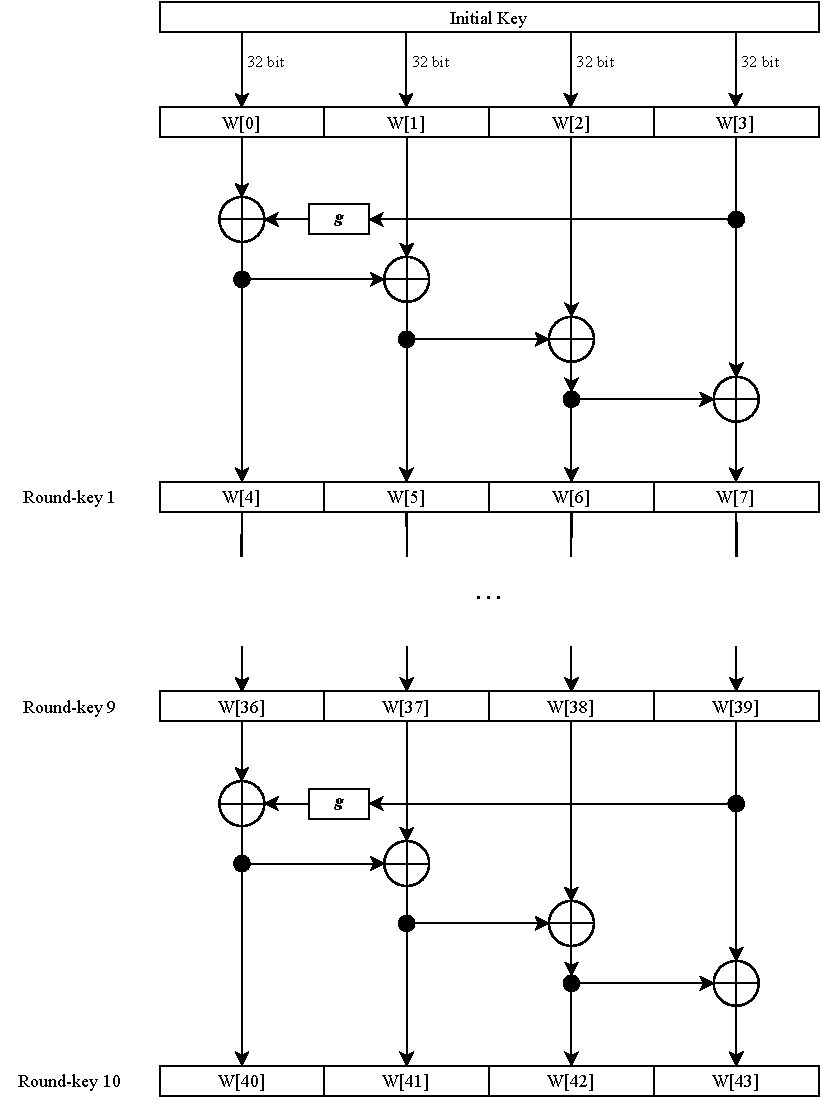
\includegraphics[width=\linewidth]{data/assets/key_expansion.pdf}
  \end{minipage}%
  \begin{minipage}{.35\textwidth}
    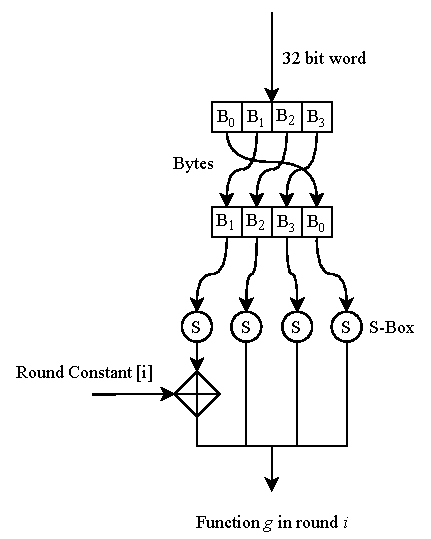
\includegraphics[width=\linewidth]{data/assets/g_function.pdf}
  \end{minipage}
  \caption{The key expansion algorithm \cite{paar}}
  \label{fig:keyexpansion}
\end{figure}


%!TEX root = thesis.tex
\chapter{Commandline Interface}
\label{commandline_interface}
The only way to interact with the program is via the commandline. In order to provide a usable interface for the user, the python module "click" is used. The module provides ways to pass command line arguments to function without a lot of code. This is achieved via the python concept knows as decorators.

Click or \enquote{Command Line Interface Creation Kit} is a python package for creating command line interfaces \cite{click}. The simplicity of the packages comes from how the cli is constructed. By adding a \lstinline{@click.command()} decorator to a function, the function becomes directly callable from the commandline. Further decorators add options, defaults, callbacks, and arguments. To combine multiple commands for a program a concept known as \enquote{groups} is used.

Click automatically generates help messages for the user. The basis for these messages are the docstrings found in the code, as well as the arguments of the functions. They either appear, when the program is run without a command (listing available commands) or when a command is run without arguments (providing documentation for the function).

In order to use the program without calling the python interpreter explicitly every time, the \lstinline|aes| script is used. It contains the shebang \lstinline|#!/usr/bin/env python3| and passes all arguments given to it to the wrapper. Because of the shebang it can be run by itself in a bash terminal (or similar like fish, zsh). If the program directory is added to the \lstinline|PATH| environment variable of the terminal session, the script can be called from anywhere by its name alone. This way of implementing runnable Python scripts is common practice. The library used for testing (pytest) uses the same concept for its executable script.


%!TEX root = thesis.tex
\section{File Structure}
The main file of the program is \lstinline|wrapper.py|. It contains the command line interface, all the setup logic, as well as the input and output handling. All non-standard python dependencies are listed within the requirements file. This way they can all be installed with one pip command. The README contains an overview over the program, as well as usage and installation instructions.


\begin{lstlisting}
wrapper.py                                    lib/
aes                                             libaes_encrypt.so
src/                                            libaes_decrypt.so
  AES_encrypt.h                               test/
  AES_encrypt.c                                 __init__.py
  AES_decrypt.h                                 test_AES_decrypt.py
  AES_decrypt.c                                 test_AES_encrypt.py
  key_expansion.py                              test_key_expansion.py
  AES_generator.py
README.md
requirements.txt
\end{lstlisting}


The source directory contains all of the AES algorithm functionality: en- and decryption of blocks, key expansion, and S-Box generation. It is structured into the source code and header files for the en- and decryption code, one python file for the key expansion, and one for the generation of lookup tables (generator). For python the directory constitutes a module that can be imported in the wrapper and testing files. All functions of the en- and decryption as well as key expansion files are explained in the appropriate sections of the documentation.


\section{Testing}
The search for a suitable test framework led to pytest, a library specifically well suited for small scale projects like this one. It made it fast and easy to write tests with multiple cases. All function inside C and python files can be tested with pytest, as the C-Code is compiled into libraries and simply called from python anyways. \cite{pytest}

\subsection{File Structure}
The test files are located in the \lstinline|tests| directory below the wrapper file, on the same level as the source directory. Tests for different parts of the program are separated out into their own files.
\begin{lstlisting}
wrapper.py
src/
test/
  __init__.py
  test_AES_decrypt.py
  test_AES_encrypt.py
  test_key_expansion.py
\end{lstlisting}
The \lstinline|__init__.py| file is empty and simply needed because of the python module types pytest can handle. During test execution pytest will look through all subdirectories and find all the import locations for the modules required for the tests.

\subsection{Structure of a Test Function}
Test functions are marked by starting with the keyword \lstinline|test| (e.g \lstinline|test_inverseShiftRows|). The pytest decorator \lstinline|mark.parametrize| can be used to define tuples of test cases. Pytest will run all cases given in the decorator against the function during execution. The function itself contains all the setup code needed to call execute the functionality to be tested. At the end of a test function is an \lstinline|assert| statement. Pytest checks for this assertion to judge the outcome of the test. The test function for the \lstinline|inverseShiftRows| as an example:
\begin{lstlisting}
@pytest.mark.parametrize(
    ('input_block', 'expected'),
    (
        ("fde596f1054737d235febad7f1e3d04e", "fde3bad205e5d0d73547964ef1fe37f1"),
        ("d1c4941f7955f40fb46f6c0ad68730ad", "d1876c0f79c4300ab45594add66ff41f"),
        ("c65e395df779cf09ccf9e1c3842fed5d", "c62fe109f75eedc3cc79395d84f9cf5d")
    )
)
def test_inverseShiftRows(input_block, expected):
    """test vector from FIPS 197 Appendix C, Round 5.is_row, istart"""
    test_block = bytearray.fromhex(input_block)
    reference = bytearray.fromhex(expected)
    byte_array = ctypes.c_ubyte * len(test_block)
    aeslib.inverseShiftRows(byte_array.from_buffer(test_block))
    assert test_block == reference
\end{lstlisting}


\subsection{Running the Test Suite}
Before execution pytest must be installed on the system. The installation process is analogous to all python packages hosted on the python package index (pypi).

To execute the test suite the \lstinline|pytest| script needs to be run from the program root (the directory \lstinline|wrapper.py| is located in). It can simply be typed into a terminal on that path. It will collect all the functions starting with the keyword \lstinline|test| and run them.

Output of a test suite execution:
\begin{lstlisting}
> pytest
================================ test session starts =================================
platform linux -- Python 3.6.9, pytest-6.2.1, py-1.10.0, pluggy-0.13.1
rootdir: /mnt/g/Software Projekte/AES/code
collected 38 items

tests/test_AES_decrypt.py ................                                     [ 42%]
tests/test_AES_encrypt.py ........s.                                           [ 68%]
tests/test_key_expansion.py ............                                       [100%]

=========================== 37 passed, 1 skipped in 1.72s ============================
\end{lstlisting}

Each dot after the test file represents successful test case, \enquote{s} denotes a skipped test case, and \enquote{f} a failed test case.



\hypertarget{functions---constant-generators}{%
\section{Functions - constant
generators}\label{functions---constant-generators}}

The following functions are from `AES\_encrypt\_generator.py' No
function in the following chapter does error checking, since they are
only intended for use inside a static, unchanging setting.

\hypertarget{galois-field-multiplication-lookup-table-generator}{%
\subsection{Galois field multiplication lookup table
generator}\label{galois-field-multiplication-lookup-table-generator}}

\hypertarget{description}{%
\subsubsection{Description}\label{description}}

As \cite{rijndael} recommends in chapter 4.1.1 Galois field multiplications
used in MixColumns were implemented as lookup tables in GFMLT. Since the
number of possible multiplication results is highly restricted in $GF(2^{8})$
the table storing all results uses neglibe memory. This avoids computing
the multiplications over and over. Furthermore in chapter 10.8.1 the
authors suggest, that implementing the multiplications as table lookups
makes the algorithm more resistant to timing attacks, since the finite
field multiplication performed in MixColumns is the only operation in
Rijdael that is not computed in constant time. In their 8-bit
implementation in chapter 4.1.1 they suggest only generating a table
where table t[a] = 02 * a, since multiplication with one is the factor
itself and multiplication with three can be efficiently archived by
XORing the result of the multiplication with two with the original
number: 03 * a = (02 * a) xor a 

To avoid leaking more timing data than
absolutely necessary the present implementation uses a lookup table for
all values, since this ensures that for each multiplication the CPU
(theoretically) does always the exact same amount of work, thus ensuring
it always takes the exact same amount of time. This size increase by 2 *
256b = 512 bytes (compared to the suggested implementation with only one
row) is negligible for our target of x86-CPU-systems, which today
typically feature memory sizes in the gigabyte range. 

\cite{rijndael} did not
make a mistake in their implementation suggestion though, since the
small lookup table variant was only suggested for memory constrained
8-bit environments. For 32-bit-architectures or wider they make even more
extensive use of lookup tables than the present implementation does
(compare ch. 4.2). This variant has not been used, since it reduces the
steps of the algorithm for each column in each round into four table
lookups accessing large tables crafted for this purpose, and four XOR
operations concatenating the lookup-results. This obscures the original
layout of the algorithm heavily and it was decided, that it should it to be recognizable
in the present implementation.

In the end the suggestions \cite{rijndael} makes regarding this topic have to
be taken with a grain of salt, since the extensive use of lookup tables
seems to enable new side channel attack vectors as previously discussed.

The lookup table used by the present implementation extends over two
dimensions: three rows for the multiplicators one, two and three and 256
columns to store the results of the multiplications with the numbers
denoting the column indices. Since the first dimension denotes the
multiplicator m, m - 1 accesses the right array for multiplication with
m, while the second dimension accesses the result for the value wanted.

\begin{quote}
The program needs to compute the multiplication of two times 114. This
means it has to access gal\_mult\_lookup[2-1]. For the result it
simply needs to use the second factor as the array index for the second
dimension. Thus the final array access to calculate 2 * 114 in $GF(2^{8})$ is
gal\_mult\_lookup[1][114]. For 3 * 86 it would be
gal\_mult\_lookup[2][86] etc.
\end{quote}

\hypertarget{implementation}{%
\subsubsection{Implementation}\label{implementation}}

\begin{lstlisting}
def mult_gal(a, b):
    """
    Multiplicates two numbers in the Galois Field specified by the AES-Standard.

    Algorithm specified under
    https://en.wikipedia.org/wiki/Finite_field_arithmetic#multiplication
    as a modiefied version of the "peasant's algorithm"
    Tested with https://www.ece.unb.ca/cgi-bin/tervo/calc2.pl
    """
    
    p = 0
    for i in range(8):
        if (a == 0) or (b == 0):
            break
        if b & 1:
            p ^= a
        b >>= 1
        a = ((a << 1)%256) ^ (-(a >> 7) & 0x1b)
    return p
\end{lstlisting}

This implementation of multiplication in $GF(2^{8})$ modulo $m(x) = x^8 + x^4 +
x^3 + x + 1$ is an adapted version from the `peasant's algorithm' as
described in
\cite{peasants}.
It takes two integers with values in range of 0-255 `a' and `b'. First
the variable `p' gets initialized with 0. The following loop gets
repeated at most eight times: If one of the two factors is 0 the
algorithm terminates. After that, `mult\_gal' evaluates, whether `b' is
odd by performing a bitwise AND-operation with `b' and 1. If the least
significant bit of `b' was toggled `p' gets XORed with `a' and the
result is stored in p. After that `b' gets bitshifted one to the right,
which equals division by two while ignoring the remainder. The last step
has two components.
The first component shifts 'a' to the right by one and cuts off any byte overflow
by using the modulo function. If such overflow occured, the modulo operation has to be
applied to the shifted 'a' in order to keep in in $GF(2^{8})$. This is done by XORing it 
with m(x) which is 100011011 in binary and 1b in hexadecimal, when fit into a byte (because
this removes the most significant digit of m(x)). To detect overflow 'a' is shifted to the right by 7
and then negated. If the most significant bit of 'a' was set (which means overflow), 1b gets ANDed
with -1 or 11111111 in binary (due to the two's complement), thus resulting in the modulo being applied to the doubled 'a'. In the other case 1b gets ANDed with 0, which results in the second term getting cancelled out, resulting in a simple doubling of 'a'.

'gen\_mult\_lookup()' then uses the function to generate the values for
multiplication of all numbers in $GF(2^{8})$ with two and three.

The results (App.XXX) were spot-checked against
https://www.ece.unb.ca/cgi-bin/tervo/calc2.pl with P(x) = 100011011.

\hypertarget{s-box-generator}{%
\subsection{S-box generator}\label{s-box-generator}}

\hypertarget{description-1}{%
\subsubsection{Description}\label{description-1}}

The S-box generator is used to generate the S-box needed in the
SubBytes-function.
The values of the AES S-box are computed by taking the value of the byte
that needs to be substituted, finding its inverse in $GF(2^{8})$ with the
irreducible polynomial $m(x) = x^8 + x^4 + x^3 + x + 1$ and applying an
affine transformation to that inverse. (\cite[ch 3.4.1]{rijndael})

\begin{figure}
\centering
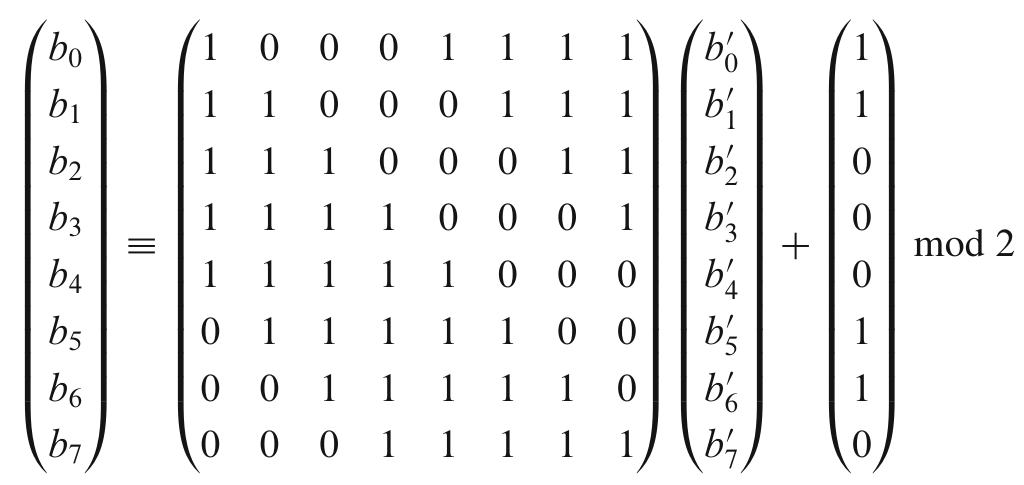
\includegraphics[scale = 0.3]{data/figures/affinetrans.png} 
\caption{The affine transformation used in the AES S-box depicted as a matrix multiplication.}
\end{figure}

The S-box contains a substitution for every value an unsigned byte is
able to contain. Fig. XXX shows the S-box filled with values (in
hexadecimal) the present implementation generates. To use it in this
table format one has to split the byte to substitute into its digits.
The most significant digit is used to look up the row, the least
significant shows the column in that row. The intersection shows the
substitution value.

\begin{quote}
The byte to substitute contains the hexadecimal value of b8. The most
significant digit is b, meaning the substitution value is located in the
b-row. The least significant digit is 8, meaning the substitution value
is located in the 8-column of the table. Therefore the substitution
value is 6c, because it is located, where the b-row and the 8-column
intersect each other.
\end{quote}

\hypertarget{implementation-1}{%
\subsubsection{Implementation}\label{implementation-1}}

\begin{lstlisting}
def mult_inv_gal():
    """
    Generates a table of the multiplicative inverse of the Elements
    contained within the AES-Galois-Field.

    It uses an unelegant brute-force-method.
    """
    list_start = [*range(1, 256)]
    list_res = [0]
    for i in range(256):
        for j in list_start:
            if mult_gal(i, j) == 1:
                list_res.append(j)
                list_start.remove(j)
    return bytearray(list_res)
\end{lstlisting}

This function generates the inverses for all values in $GF(2^{8})$. First it
generates a list with the values from 1 to 255. After that it creates
another list containing the element 0 (since 0 has no inverse). Now it
iterates through all 256 possible values p. For each p it goes through
`list\_start' and multiplies them in $GF(2^{8})$ modulo m(x) using the
previously mentioned `mult\_gal' function. Since multiplying a number x
with its inverse always results in the multiplicative identity 1, the
present implementation simply tries to multiply all elements in $GF(2^{8})$
with each other (basically a brute-force approach) to see if the product
equals 1. In that case the value r from `list\_start' is appended to
`list\_res' at the index of the current value of p. After that r is
removed from list\_start, since every p has only one inverse in $GF(2^{8})$
modulo m(x) (proven experimentally by multiplying all elements in $GF(2^{8})$
with each other and noting the occurrences of products equal 1). In the
end the function returns `list\_res' converted to a byte array,
containing numbers that are the inverses of the values of their indices
(eg. element in listindex 37 is the inverse to the number 37).

\begin{lstlisting}
def shift_left(byte, rot):
    """Implements a left bitwise circular shift for bytes."""
    temp = (byte << rot)%256
    byte = temp | ((byte >> (8-rot)))
    return byte
\end{lstlisting}

This function implements a left bitwise circular shift of a byte. It
takes two arguments, `byte' and `rot'. `byte' is an integer in the range
of 0-255 and rot is an integer, denoting the number of places `byte'
should be shifted by. It starts by applying a bitwise left shift to
`byte', shifting it `rot' times. The result is reduced by modulo 256,
since the result cannot leave the range denoted by an unsigned byte,
e.g. 0-255. The reduced result is placed into the variable `temp'. Now
the bits of `byte' that got shifted to the left and `cut off' by the
modulo operation have to be brought back to the right. For that we shift
`byte' 8 - `rot' bits to the right. Now the two `halves' get combined by
applying a bitwise OR to `temp' and the result of the rightshift. This
result is saved in `byte'. Finally the function returns `byte'.

\begin{lstlisting}
def gen_sbox():
    """Genereates the AES S-box"""
    mult_inv_table = mult_inv_gal()
    sbox = bytearray(256)
    j = 0
    for i in mult_inv_table:
        #affine transformation
        sbox[j] = i ^ shift_left(i, 1) ^ shift_left(i, 2) ^ shift_left(i, 3) ^ shift_left(i, 4) ^ 0x63
        j += 1
    return sbox
\end{lstlisting}

This function generates the S-box array. First it uses the
`mult\_inv\_gal' function to generate a list containing all
multiplicative inverse of the elements in $GF(2^{8})$. After that it
allocates a byte array with length 256 called `sbox' and initializes the
variable `j' with zero. Then it iterates through the array of inverses,
applying the affine transformation and storing the result in sbox. The
affine transformation is computed by XORing the list element with
versions of itself that have been shifted left via circular byteshift
one, two, three and four times. Finally the result gets XORed with 99 to
obtain the result of the transformation.
(https://en.wikipedia.org/wiki/Rijndael\_S-box\#forward\_s-box) The
function finishes by returning the S-box-byte-array.

Since this is a static function generating always the same array, the
resulting array was compared once with the table in \cite[Fig. 7](fips197)

\hypertarget{functions---encryption}{%
\section{Functions - encryption}\label{functions---encryption}}

The following functions are from `AES\_encrypt.c'
(`Implementation'-chapters). The following chapter is based on \cite{fips197} and the authors own
knowledge/opinions, if not mentioned otherwise.

\hypertarget{key-addition}{%
\subsection{Key Addition}\label{key-addition}}

\hypertarget{description-2}{%
\subsubsection{Description}\label{description-2}}

\begin{figure}
\centering
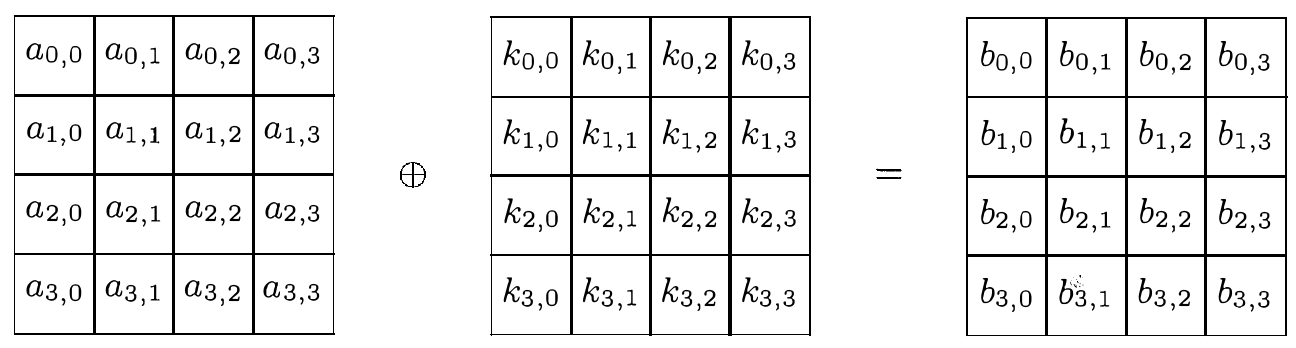
\includegraphics[scale = 0.3]{data/figures/addroundkey.png} 
\caption{Addition of the round key to to the state via bitwise XOR. a0,0 xor k0,0 = b0,0 etc.}
\end{figure}

In this transformation a round key is
combined with the state, thus modifying it. The combination is
accomplished using the bitwise XOR operation. The round key array is
derived from the initial cipher key using the key schedule. Containing
16 bytes, each round key is equally long to a block. Since there are N+1
round keys generated (where N is the number of rounds), each round uses
a different round key (5.1.4).

\hypertarget{implementation-2}{%
\subsubsection{Implementation}\label{implementation-2}}

\begin{lstlisting}
/*
 * Adds the roundkey to a block.
 */
inline void AddRoundKey(uint8_t * restrict bytes, 
                        const uint8_t * restrict keys)
{
        for(uint8_t i = 0; i < 16; i++) {
                bytes[i] ^= keys[i];
        }
}
\end{lstlisting}

This function is used to add the current round key to the current block.
It takes a restricted pointer to the first byte of the block the cipher
is currently operating on and a restricted pointer to a constant, which
points to the first byte of the round key, that is supposed to be used
currently. It proceeds to combine each of the sixteen bytes of the block
with a corresponding byte of the round key designated to the current
round using the bitwise XOR. The result is then stored in the block byte
used in the XOR operation, meaning that first byte one of the block will
be XORed with byte one of the round key and then the result will be
stored in place of byte one and so forth for all sixteen bytes.

Since the function is relativly short the `inline'-keyword is used to
save the overhead of an additional function call in tradeoff with a
bigger binary.

\hypertarget{shift-rows}{%
\subsection{Shift rows}\label{shift-rows}}

\hypertarget{description-3}{%
\subsubsection{Description}\label{description-3}}

\begin{figure}
\centering
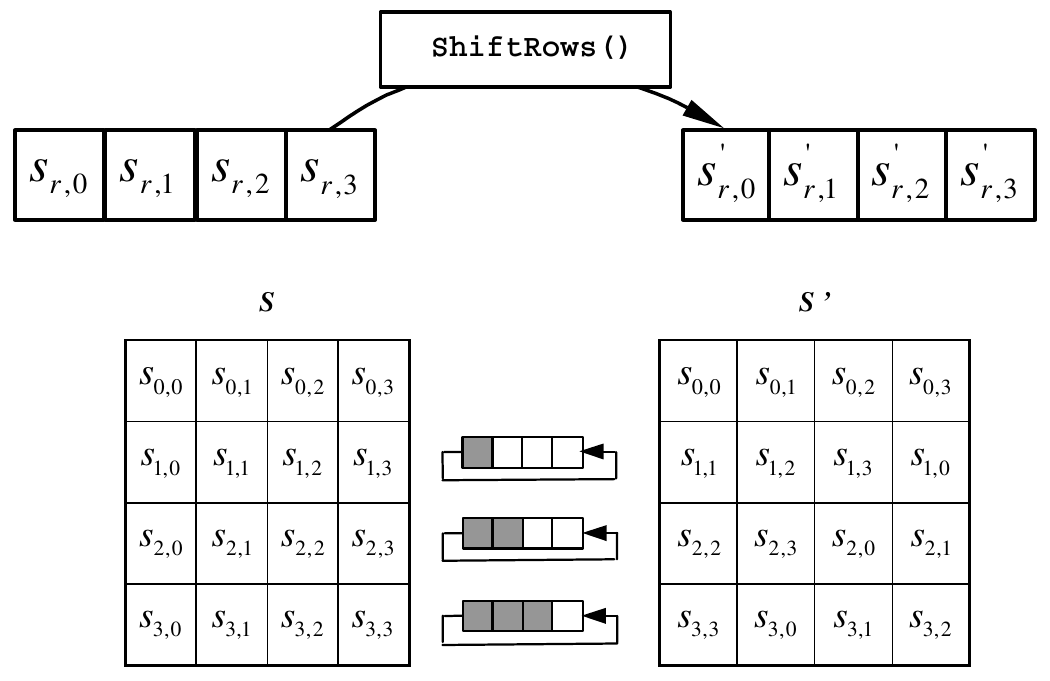
\includegraphics[scale = 0.3]{data/figures/shiftrows.png} 
\caption{The ShiftRows-transformation "rotates" the rows of the state (left) by different offsets, resulting in the state on the right}
\end{figure}

(rijndael)(p.37) states, that this transformation of the state represents a byte transposition, using
cyclical shifts with different offsets. The first row of the 4x4-Matrix
of 16 bytes that constitutes the so called state is not shifted at all,
the second row by one step to the left, the third row uses two steps and
the fourth row three.

According to (rijndael) this transformation step is needed to ensure
optimal diffusion of the state. The diffusion is supposed to protect
against differential and linear cryptanalysis. The authors further
elaborate, that in order to archive optimal diffusion all
offsets of the cyclical shifts have to be different.

Since there are multiple possibilities for different offsets and not all
of them provided equal protection studies of attacks against Rijndael
were analyzed. From the offsets that proved to be the most resistant the
simplest offset was chosen.

\hypertarget{implementation-3}{%
\subsubsection{Implementation}\label{implementation-3}}

\begin{lstlisting}
/*
 * Achieves the AES-ShiftRows by representing it as a series of array-assignments.
 */
void ShiftRows(uint8_t * restrict block, uint8_t * restrict tempblock)
{
        memcpy(tempblock, block, 16 * sizeof(uint8_t));

        block[1] = tempblock[5];
        block[2] = tempblock[10];
        block[3] = tempblock[15];
        block[5] = tempblock[9];
        block[6] = tempblock[14];
        block[7] = tempblock[3];
        block[9] = tempblock[13];
        block[10] = tempblock[2];
        block[11] = tempblock[7];
        block[13] = tempblock[1];
        block[14] = tempblock[6];
        block[15] = tempblock[11];
}
\end{lstlisting}

The function ShiftRows performs the ShiftRows-transformation on the
state. It takes a restricted pointer to the first byte of the block the
cipher is currently operating on and a restricted pointer to a temporary
block. First the content of the block is copied into the array the
tempblock-pointer is marking. After that the row shifts are represented
by assigning the bytes into their positions in the block after the
shifts from the tempblock,

\hypertarget{mix-columns}{%
\subsection{Mix columns}\label{mix-columns}}

\hypertarget{description-4}{%
\subsubsection{Description}\label{description-4}}

The MixColumns-transformation is called a bricklayer permutation by
(rijndael). The authors
mention multiple design criteria, they deemed important for this
particular transformation:

\begin{enumerate}
\def\labelenumi{\arabic{enumi}.}

\item
  \emph{The bricklayer transformation is supposed to operate on columns
  containing 4 bytes.} This aspect is supposed to aid with the optimal
  implementation of look-up tables on 32-bit architectures, thus
  ensuring a speedy computation of the transformation.
\item
  \emph{The operation should be linear over GF(2)}, meaning the Galois
  Field of the two elements 0 and 1. This property aides the authors in
  their so-called `Wide Trail Strategy' (p.126) which is supposed to
  protect against differential and linear cryptanalysis.
\item
  \emph{The diffusion achieved by this transformation is supposed to
  have ``relevant'' power.} The third property is again supposed to
  support the `Wide Tail Strategy'.
\item
  \emph{The authors put emphasis on the performance of this step on 8-bit
  CPUs.} They deemed this neccessary, as they feared that the MixColumns
  transformation would be ``the only step that good performance on 8-bit
  processors is not trivial to obtain for.''(p.39)
\end{enumerate}


\begin{figure}
\centering
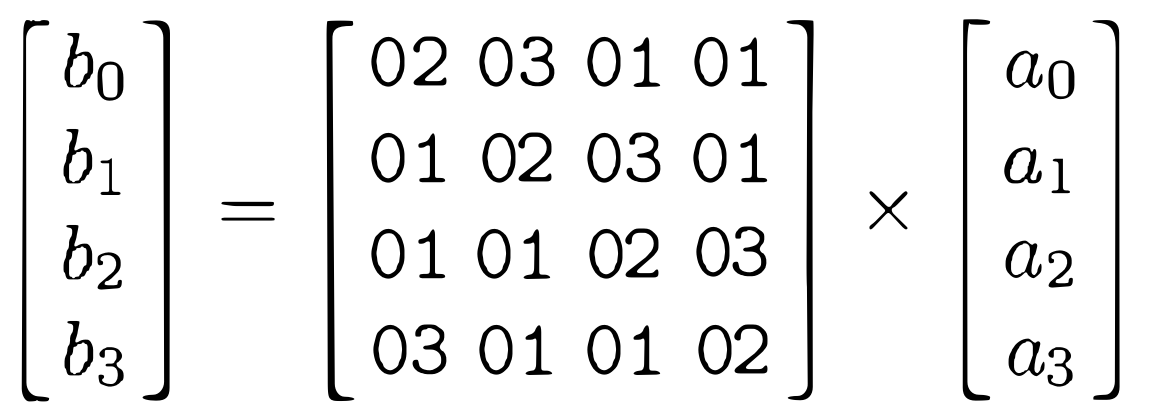
\includegraphics[scale = 0.2]{data/figures/mixcolumn.png} 
\caption{The MixColumns-transformation, represented as matrix multiplication.}
\end{figure}

The transformation itself partitions the
state-matrix into four columns. Each of those columns is transformed
independently from the other three. A single column acts as a polynomial
over $GF(2^{8})$, which is multiplied modulo $x^4 + 1$ with a fixed polynomial. In
order to meet the aforementioned criteria regarding performance,
diffusion and to fullfill the additional condition of creating an
invertible transformation (in regards to encryption) the authors were
forced to impose conditions on the fixed polynomials (rijndael). For
example, performance was archived by using only simple values for the
coefficients of the fixed polynomial. The fixed polynomial c(x) Daemen
and Rijmen settled on is $c(x) = 03 * x^3 + 01 * x^2 + 01 * x + 02$. They
state, that since c(x) and the aforementioned modulo $x^4+1$ are coprime
the calculation is invertible. The matrix-multiplication, which is seen
in Fig XXXX, is a representation of the modular multiplication with a
fixed polynomial.

158 - 88 4.1.1. 

\hypertarget{implementation-4}{%
\subsubsection{Implementation}\label{implementation-4}}

\begin{lstlisting}
/*
 * Achieves the AES-MixColumns by representing each result byte as a series of
 * table-lookups XORed with each other.
 */
void MixColumns(uint8_t * restrict block, uint8_t * restrict tempblock, 
                const uint8_t (* restrict gal_mult_lookup)[256])
{
        memcpy(tempblock, block, 16 * sizeof(uint8_t));

        for(uint8_t i = 0; i < 16; i += 4) {

                block[i] = gal_mult_lookup[1][tempblock[i]] ^
                        gal_mult_lookup[2][tempblock[i+1]] ^
                        gal_mult_lookup[0][tempblock[i+2]] ^
                        gal_mult_lookup[0][tempblock[i+3]];

                block[i+1] = gal_mult_lookup[0][tempblock[i]] ^
                        gal_mult_lookup[1][tempblock[i+1]] ^
                        gal_mult_lookup[2][tempblock[i+2]] ^
                        gal_mult_lookup[0][tempblock[i+3]];

                block[i+2] = gal_mult_lookup[0][tempblock[i]] ^
                        gal_mult_lookup[0][tempblock[i+1]] ^
                        gal_mult_lookup[1][tempblock[i+2]] ^
                        gal_mult_lookup[2][tempblock[i+3]];

                block[i+3] = gal_mult_lookup[2][tempblock[i]] ^
                        gal_mult_lookup[0][tempblock[i+1]] ^
                        gal_mult_lookup[0][tempblock[i+2]] ^
                        gal_mult_lookup[1][tempblock[i+3]];
        }
}
\end{lstlisting}

The function MixColumns takes multiple arguments. First it takes a
restricted pointer to the first byte of the block the cipher is
currently operating on, followed by a restricted pointer to a temporary
block and lastly the function gets a restricted pointer to the constant,
multi-dimensional GFMLT. MixColumns starts by copying the current state
from `block' into `tempblock'. After that it iterates through every row
by processing 4 consecutive bytes at a time, before it moves to the
following for consecutive bytes of `block'. Each Byte in `block' becomes
the result of four Galois field multiplications combined through the
bitwise XOR-operation, which represents the Galois field addition. The
multiplications are implemented as lookups in the GFMLT and combine the
coefficients of the fixed polynomial c(x) with the bytes of the current
row. After processing all four rows and returning, MixColumns has
written the results of this transformation in place of the current block
being processed.

\hypertarget{substitute-bytes}{%
\subsection{Substitute bytes}\label{substitute-bytes}}

\hypertarget{description-5}{%
\subsubsection{Description}\label{description-5}}

\begin{figure}
\centering
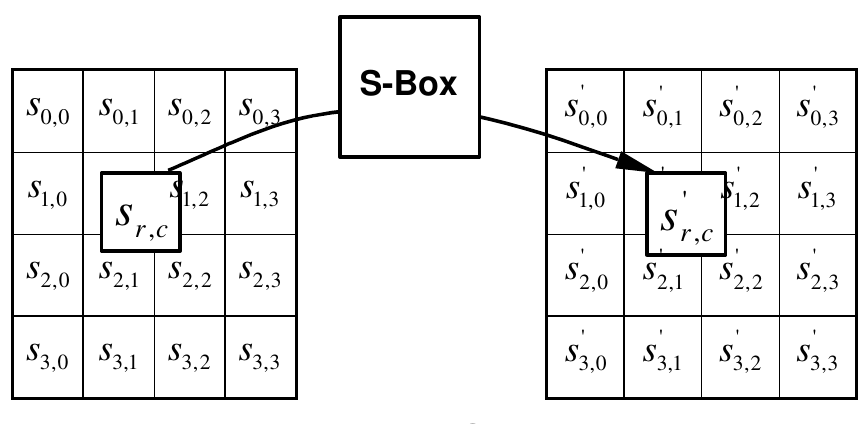
\includegraphics[scale = 0.3]{data/figures/subbytes.png}
\caption{SubBytes applies the S-box substitution to every byte of the
state}
\end{figure}

Being the only non linear transformation, SubBytes is labeled a
bricklayer permutation by (rijndael) that applies byte substitution to
each byte of the state. This substitution is facilitated throught the
AES Sbox. AES uses
only this one Sbox, although the authors mention, that Rijndael ``could
as easily be defined with different S-boxes for every byte.'' (p.35).
They descided against it, because one key criteria during the
developement process for them was simplicity (ch.~5.2). Rijmen and
Daemen argue, that simplicity is an important contributer towards a
correct implementation, that it helps to get more people to review it,
since it is easier than reviewing more complex software and that it may
aide the notion it is easier to attack, thus motivating more of such
attacks. They further elaborate that the latter two points contribute to
the cryptographic credebility of the algorithm, especially if out of
many tries no successful attack can be mounted. Furthermore simpicity as
a design criterion was used to balance the security with the factors
efficiency and versatility. This simplicity was partially archived by
designing the algorithm following the principle of what they call
``symmetry''. Their tenet of symmetry within the round transformation
(ch.~5.3.2) " implies that it treats all bits of the state in a similar
way." (p.66). They explain that this imposes some restrictions, amongst
others the requirement to use only one S-box for the whole state in their
non-linear step. Symmetry across all rounds (ch.~5.31.) dictates that
all rounds have to be identical. This keeps the specification and
implementation short, since only one round has to be described/expressed
in code. This tersness in definition is also of benefit for hardware
implementations, since there has to be only one circuit designed to
implement all rounds, instead of one circuit per round. The other consequence is,
that only one S,box can be used for all rounds
(contrary to DES (XXX)).

\hypertarget{implementation-4}{%
\subsubsection{Implementation}\label{implementation-4}}

\begin{lstlisting}
/*
 * Substitutes all bytes in a block with bytes from a sbox.
 */
inline void SubBytes(uint8_t * restrict bytes, const uint8_t * restrict sbox)
{
        for(uint8_t i = 0; i < 16; i++) {
                bytes[i] = sbox[bytes[i]];
        }
    
}
\end{lstlisting}

The SubBytes-implementation is pretty straightforward. The function
recieves two restricted pointers, one called `bytes', pointing to the
first byte of the current state, and one pointer to a constant array,
which contains the sbox to be used. The function now iterates through
`bytes', assigning every element from that array a new value by
accessing the element of the `sbox'-array, which corresponds to the
value in the current `bytes' element.

\hypertarget{full-block-encryption}{%
\subsection{Full block encryption}\label{full-block-encryption}}

\hypertarget{description-6}{%
\subsubsection{Description}\label{description-6}}

To encrypt one block of AES the whole cipher with all rounds has to be
executed. One round consists of four steps, which represent the four
transformation employed in the encryption algorithm. Those transformations are (in that order) SubBytes, ShiftRows, MixColumns and AddRoundKey.
If N is the number of rounds specified by the encryption standard then
the algorithm will execute N-1 * r, while the Nth round omits the
MixColumns step, but is otherwise identical. Before the first round one
additional AddRoundKey is performed on the state.

\hypertarget{implementation-5}{%
\subsubsection{Implementation}\label{implementation-5}}

\begin{lstlisting}
void encryptBlock(uint8_t * restrict block, uint8_t * restrict tempblock, 
                  const uint8_t * restrict keys, const uint8_t rounds, 
                  const uint8_t * restrict sbox, 
                  const uint8_t (* restrict gal_mult_lookup)[256])
{   
        uint8_t ikeys = 0;
        AddRoundKey(block, keys);
        ikeys += 16;

        for(uint8_t i = 0; i < rounds - 1; i++) {   
                SubBytes(block, sbox);
                ShiftRows(block, tempblock);
                MixColumns(block, tempblock, gal_mult_lookup);
                AddRoundKey(block, &keys[ikeys]);
                ikeys += 16;
        }
        
        SubBytes(block, sbox);
        ShiftRows(block, tempblock);
        AddRoundKey(block, &keys[ikeys]);
}
\end{lstlisting}

The present implementation of the Cipher takes multiple arguments. Like
in all other functions a restricted pointer to the first element in the
state array is provided. The second argument is a restricted pointer to
another bytearray of length sixteen, that can be used to store temporary
values. The third argument is a restricted pointer to a constant
bytearray, which contains the roundkeys. The next argument is a constant
byte denoting the number of rounds for the algorithm. It is passed to
provide future extensebility in case different key lengths are used and
thus different round numbers are needed, since this number depends on
the key length. The fifth argument is a restricted pointer to a constant
array containing the S-box values. The last argument is a restricted
pointer to a constant, multidimensional array containing the GLFMLT.

The function begins by allocating an unsigned byte on the stack and
assigning it the value of zero. This variable keeps track of the first
byte of the next key that is to be used in the function AddRoundKey,
thus has to be incremented by 16 after every call to the
AddRoundKey-function. The name is derived from ``\textbf{i}ndex of the
round\textbf{keys}''. Next the AddRoundKey-function is called with the
pointer to the current state and a pointer to the first round-key, which
is followed by the first increase of the `ikeys'-variable. Now the
rounds are executed in a for-loop, that counts from zero to the number
of rounds minus one. Every round consists of the following steps:
SubBytes is called with a pointer to the current state and a pointer to
the sbox, followed by a call of ShiftRows with a pointer to the current
state and the tempblock, then a call of MixColumns with pointers to the
current state, the temporary block and the GFMLT. Now comes a call to
AddRoundKey with a pointer to the current state and the memory address
`keys' would point towards, if it was increased by the amount stored in
`ikeys'. The latter passes on the starting address of the bytearray of
the next round key to be used by AddRoundKey. The last part of each
round is the increase of the `ikeys'-counter. After exiting the loop the
function executes one more round without the call to MixColumns and the
increase of the `ikeys'-counter variable and then it returns.

\hypertarget{encryption-of-multiple-consecutive-blocks}{%
\subsection{Encryption of multiple consecutive
blocks}\label{encryption-of-multiple-consecutive-blocks}}

\hypertarget{description-7}{%
\subsubsection{Description}\label{description-7}}

Although not explicitly required in context of this work, the present
implementation contains the possibility to encrypt multiple consecutive
blocks. With that it enables encryption of for example messages larger
than sixteen bytes or even files. 

(paar) (ch.~5.1.1) describes
encryption schemes like found in the present implementation the simplest
block cipher modes of operation, called `Electronic Codebook Mode'  (ECB).
Every cipher block is generated by simply encrypting the plaintext with
the round keys and appending the encrypted blocks. The first advantage
of this method is that no synchronization between the en- and decrypting
party is necessary, since each block can be processed independently of
each other. Bit errors do not propagate through the whole ciphertext but
are confined to the block they occured in. The implementation has also
the potential to become very fast, thanks to the posibility of
processing different blocks on different cores, thus enabling
parallelisation of en- and decryption. 

The weaknesses of this mode
should not be underestimated though. Due to the fact that every block is
encrypted with the same key, the same plaintexts will generate the same
outputs. If the ciphertext is examined at a block level this is not of
greater significance, since AES guarantees that each encrypted block is
indistinguishable from randomly generated bytes. But if the plaintext as
a whole gets analyzed patterns may emerge. Those patterns leak
information about what parts of the plaintext contain the same 128-bit
sequence, because those parts also share a (different) bit seqence in
the corresponding ciphertext. Furthermore, a third party watching an
exchange encrypted in ECB can tell, when the same
message is send twice, or if the header of different messages is the
same, for examle if each message was using the same salutation. (paar)
demonstrates two attack avenues, that are a direct result of ECB. The
first one exploits the ECB-encrypted communication channel between two
banks. Here the attacker A just needs to open one account on both banks
and review the communication channel for patterns from test transactions
he is sending between the two accounts. If the banks do not rotate keys
A will soon know which encrypted blocks belong to his account number and
which block denote the recieving account. After learning that they can
exchange all blocks they know as reserved for the number of the
recieving account with the blocks for their own account number and
divert all transactions between the two banks to A's account. The other
attack avenue is the emergence of patterns visible to the naked eye. For
this example we created an image in the bitmap format(Fig. XXX). This
image was encrypted with a modified variant of the present
implementations file encryption mode \footnote{Encrypted with the following settings for key generation: key = "passwort", iterations = 20, salt = "aeskurs"}. The modification (inserted just
before the while-loop) ensures that the header of the .bmp-file is
preserved and not corrupted by the encryption. It reads the first 55
bytes (since the header is 54 bytes long
(https://www.daubnet.com/en/file-format-bmp)) and writes them to the
encrypted file without encrypting them. After that, the rest of Fig. XXX
is read, encrypted and appended. The result Fig. XXX, albeit encrypted
with an algorithm concidered secure, shows a clear and readable pattern.
For comparison we used the `pyaes'-library to encrypt the image in the
same way with the same key\footnote{Encrypted with the following settings for key generation: key = "passwort", iterations = 20, salt = "aeskurs"} and preservation method of the header, but
applied the Counter Mode of Operation. The result, displayed in Fig.
XXX, demonstrates, that any visible pattern resulting from
ECB-encryption disappears with the right Block Cipher Mode of Operation.
(paar)(ch.5.1.5) describes how the Counter Mode is an example of block
cipher modes of operation that avoids such patterns. First an
initialization vector IV gets choosen. This ensures that every
encryption pass is as unique as the IV. Due to this fact it is
recommended to never reuse the IV. This IV is then concatenated counter.
This combination with the length of 128 bits is then encrypted with AES
and the password. The result is XORed with 128 bits of plaintext to
create the ciphertext. The counter is increased for each concecutive
block that needs to be encrypted. This way each block of plaintext is
XORed with an uniqe combiation of IV, nonce and key. This makes it
highly unlikely for two identical blocks of plaintext to be encrypted
into two identical blocks of ciphertext, thus avoiding leakage of
information.

The present implementation is required to use ECB, since it has to be
able to reproduce the testvectors from (fips197). Due to time constraints
it was decided not to implement two different block cipher modes of
operation.

\begin{figure}
\centering
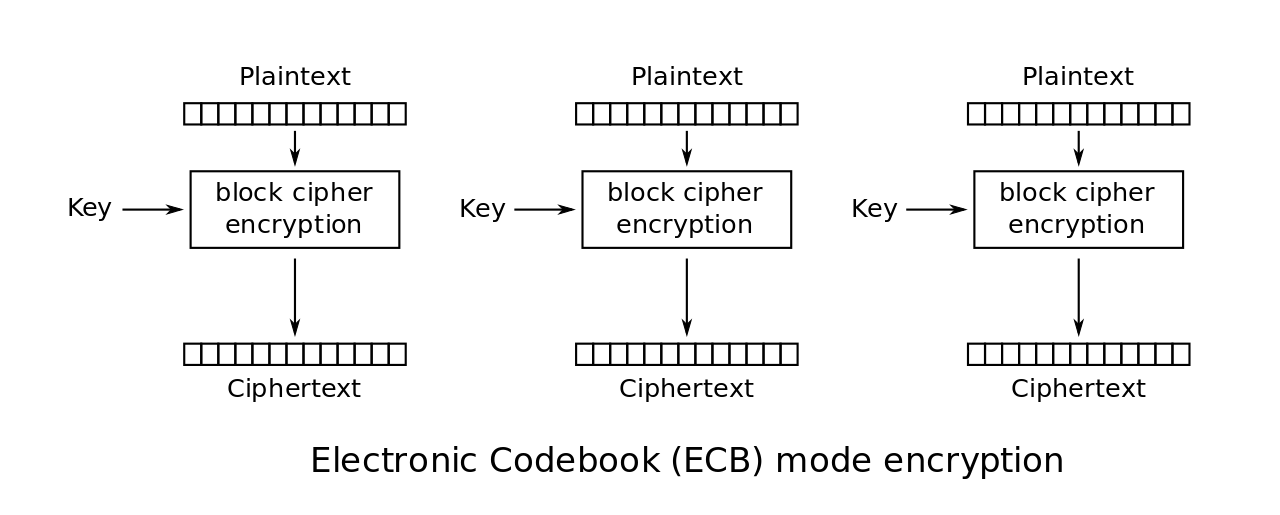
\includegraphics[scale = 0.25]{data/figures/ECB_encryption.png}
\caption{ECB: Every block of plaintext is simply encrypted with a key.}
\end{figure}

\begin{figure}
\centering
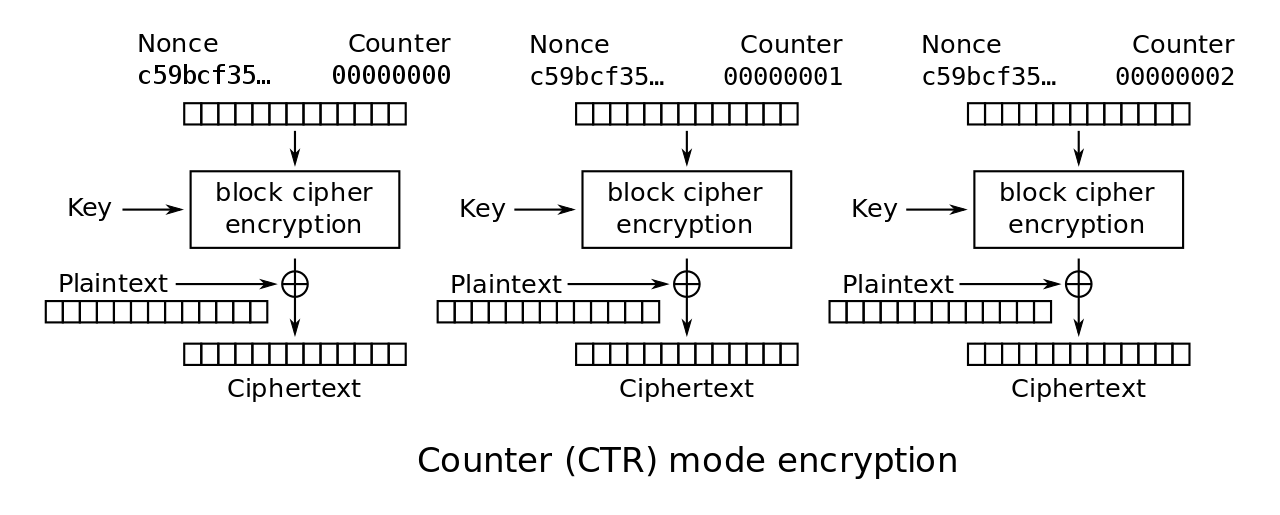
\includegraphics[scale = 0.25]{data/figures/CTR_encryption.png}
\caption{CTR: Every block of plaintext is XORed with a combination of initialization vector (here: Nonce) and counter, encrypted by the key to form the ciphertext.}
\end{figure}

In order for Electronic Codebook Mode to work correctly the bye array
containing the plaintext has to be padded though, as only byte arrays
with length l can be processed where l modulo 16 equals 0. Padding can
be implemented in multiple ways, this implementation does it as follows:

\begin{lstlisting}
def pad_input(ba):
    """pads bytearray to have a length % 16 = 0"""
    topad = 16 - len(ba) % 16
    if topad == 0:
        topad = 16 #ensures that last byte is always padding
    padding = bytearray([topad] * topad) # PKCS 5, 7
    return ba + padding
\end{lstlisting}

First it decides how many bytes the passed array is missing until the
length l of the array fulfills the requirement l modulo 16 equals 0. The
number of missing elements m is then appended m times to the array in
need of padding. If no padding is required a whole block gets padded.
This ensures the last byte of the decrypted string always contains the
information on how many bytes are padded and need to be removed, since
without this procedure a value for the last byte of one would be
ambiguous: does the last byte need to be removed since it is padding of
one or is it part of the message? This follows the concept of (PKCS \#7
RFC2315).

\begin{quote}
The array containing the plaintext is 357 bytes long. Since 357 modulo 16 = 5,
five bytes need to be added to the plaintext array. The present
implementation then adds an array containing the values \{5, 5, 5, 5,
5\} to the array.
\end{quote}

\hypertarget{implementation-6}{%
\subsubsection{Implementation}\label{implementation-6}}

\begin{lstlisting}
/*
 * Initializes the constant tables sbox, galois-field-multiplication-lookup and keys.
 * Performs AES-encryption on multiple, consecutive blocks.
 */
void encryptAES(uint8_t * restrict bytes, uint8_t * restrict initval, 
                   const size_t bytecount, const uint8_t rounds)
{   
        uint8_t sbox[256];
        uint8_t gal_mult_lookup[3][256];
        for(size_t i = 0; i < 256; i++) {
                sbox[i] = *initval++;
        }
        for(size_t i = 0; i < 3; i++) {
                for(size_t j = 0; j < 256; j++) {
                gal_mult_lookup[i][j] = *initval++;
                }
        }
        
        const uint8_t *keys = initval;
        uint8_t tempblock[16];
        
        for(size_t i = 0; i < bytecount; i += 16) {
                encryptBlock(&bytes[i], tempblock, keys, 
                             rounds, sbox, gal_mult_lookup);
        }
}
\end{lstlisting}

The function takes four arguments. The first one is a restricted pointer
to an array containing the bytes that need to be encrypted. The second
argument is a restricted pointer to an array containing the
initialization values: first the elements of the S-box, followed by the
bytes of the GFMLT, while the rest are the bytes of the round keys. The
third is a constant unsigned variable which width equals the wordwidth
of the CPU architecture the source code gets compiled on. The last
argument is a constant byte containing the number of rounds. The
function starts by allocation an array of 256 unsigned bytes called
`sbox'. After that another array named `gal\_mult\_lookup' is allocated,
but this time it is two-dimensional, using three times 256 unsigned
bytes. The name is derived from `\textbf{Gal}ois field
\textbf{mult}iplication \textbf{lookup}table'. Both are initalized with
the three following for-loops. The first loop reads the first 256 bytes
from `initvar' and assigns them to `sbox'. The following two nested
for-loops iterate through the two dimensions of `gal\_mult\_lookup' and
assign the results of the Galois field multiplications in $GF(2^{8})$ to the
respective dimensions of the array.

After populating the arrays the pointer has moved far enough through
`initvals' that it now points to the first byte of the first round key.
To make this more clear and to enable possible compiler optimizations we
create a new pointer named `keys' poining to a constant array, which is
in this case `initvals'. All future accesses to this array will be
throught `keys' or descendants of this pointer. The last step before
starting the encryption routine is the creation of an array of sixteen
unsigned bytes called `tempblock'. The next for loop starts the
encryption. Every iteration processes one block and increments the loop
index variable by sixteen, so that it can point to the next block to be
processed. In every iteration of this loop the function `enrcryptBlock'
is called with the address of the current block to encrypt, a pointer to
the temporary block, a pointer to the array containing the round keys, a
variable containing the number of rounds, a pointer to the sbox and a
pointer to the GFMLT.

Since parallelisation of the de- and encryption routine seems to be a
worthwhile endeavour for the future, this function was already designed
with that in mind. An allocation of the temporary block as a local
variable instead of a global one avoids the need for thread
synchronization, since every thread would use their own temporary block,
if every thread spawned would use this function as a starting point.


´


\appendix
%!TEX root = thesis.tex
%This is only relevant for TeXShop
\chapter{Appendix A}
\label{ch:appendixa}

\begin{figure}[h]
\centering
\includegraphics[width=\textwidth]{data/figures/aes.png}
\caption{The unencrypted bitmap-file converted to a .png-file.}
\label{fig:aespng}
\end{figure}

\begin{figure}[h]
\centering
\includegraphics[width=\textwidth]{data/figures/aesECB.png}
\caption{The bitmap-file encrypted with AES in ECB mode and converted to a .png-file. The writing "Advanced Encryption Standard" is clearly readable, despite the encryption.}
\label{fig:aesecbpng}
\end{figure}

\begin{figure}[h]
\centering
\includegraphics[width=\textwidth]{data/figures/aesCTR.png}
\caption{The bitmap-file, encrypted with AES in CTR mode and converted to a .png-file. To the naked eye the content of the picture is indistinguishable from noise.}
\label{fig:aesctrpng}
\end{figure}


\begin{table}[h]
  \resizebox{\textwidth}{!}{%
  \begin{tabular}{c | c c c c c c c c c c c c c c c c c}
    & 0 & 1 & 2 & 3 & 4 & 5 & 6 & 7 & 8 & 9 & a & b & c & d & e & f \\ \hline
    0 & 0x63 & 0x7c & 0x77 & 0x7b & 0xf2 & 0x6b & 0x6f & 0xc5 & 0x30 & 0x01 & 0x67 & 0x2b & 0xfe & 0xd7 & 0xab & 0x76 \\  1 &  0xca & 0x82 & 0xc9 & 0x7d & 0xfa & 0x59 & 0x47 & 0xf0 & 0xad & 0xd4 & 0xa2 & 0xaf & 0x9c & 0xa4 & 0x72 & 0xc0 \\ 2 &  0xb7 & 0xfd & 0x93 & 0x26 & 0x36 & 0x3f & 0xf7 & 0xcc & 0x34 & 0xa5 & 0xe5 & 0xf1 & 0x71 & 0xd8 & 0x31 & 0x15 \\ 3 & 0x04 & 0xc7 & 0x23 & 0xc3 & 0x18 & 0x96 & 0x05 & 0x9a & 0x07 & 0x12 & 0x80 & 0xe2 & 0xeb & 0x27 & 0xb2 & 0x75 \\ 4 & 0x09 & 0x83 & 0x2c & 0x1a & 0x1b & 0x6e & 0x5a & 0xa0 & 0x52 & 0x3b & 0xd6 & 0xb3 & 0x29 & 0xe3 & 0x2f & 0x84 \\ 5 & 0x53 & 0xd1 & 0x00 & 0xed & 0x20 & 0xfc & 0xb1 & 0x5b & 0x6a & 0xcb & 0xbe & 0x39 & 0x4a & 0x4c & 0x58 & 0xcf \\ 6 & 0xd0 & 0xef & 0xaa & 0xfb & 0x43 & 0x4d & 0x33 & 0x85 & 0x45 & 0xf9 & 0x02 & 0x7f & 0x50 & 0x3c & 0x9f & 0xa8 \\ 7 & 0x51 & 0xa3 & 0x40 & 0x8f & 0x92 & 0x9d & 0x38 & 0xf5 & 0xbc & 0xb6 & 0xda & 0x21 & 0x10 & 0xff & 0xf3 & 0xd2 \\ 8 & 0xcd & 0x0c & 0x13 & 0xec & 0x5f & 0x97 & 0x44 & 0x17 & 0xc4 & 0xa7 & 0x7e & 0x3d & 0x64 & 0x5d & 0x19 & 0x73 \\ 9 & 0x60 & 0x81 & 0x4f & 0xdc & 0x22 & 0x2a & 0x90 & 0x88 & 0x46 & 0xee & 0xb8 & 0x14 & 0xde & 0x5e & 0x0b & 0xdb \\ a & 0xe0 & 0x32 & 0x3a & 0x0a & 0x49 & 0x06 & 0x24 & 0x5c & 0xc2 & 0xd3 & 0xac & 0x62 & 0x91 & 0x95 & 0xe4 & 0x79 \\ b & 0xe7 & 0xc8 & 0x37 & 0x6d & 0x8d & 0xd5 & 0x4e & 0xa9 & 0x6c & 0x56 & 0xf4 & 0xea & 0x65 & 0x7a & 0xae & 0x08 \\ c & 0xba & 0x78 & 0x25 & 0x2e & 0x1c & 0xa6 & 0xb4 & 0xc6 & 0xe8 & 0xdd & 0x74 & 0x1f & 0x4b & 0xbd & 0x8b & 0x8a \\ d & 0x70 & 0x3e & 0xb5 & 0x66 & 0x48 & 0x03 & 0xf6 & 0x0e & 0x61 & 0x35 & 0x57 & 0xb9 & 0x86 & 0xc1 & 0x1d & 0x9e \\ e & 0xe1 & 0xf8 & 0x98 & 0x11 & 0x69 & 0xd9 & 0x8e & 0x94 & 0x9b & 0x1e & 0x87 & 0xe9 & 0xce & 0x55 & 0x28 & 0xdf \\ f & 0x8c & 0xa1 & 0x89 & 0x0d & 0xbf & 0xe6 & 0x42 & 0x68 & 0x41 & 0x99 & 0x2d & 0x0f & 0xb0 & 0x54 & 0xbb & 0x16 \\
  \end{tabular}
  }
  \caption{Sbox}
  \label{sbox}
\end{table}


\pagestyle{scrplain} % turn off headers and footers
% generate list of figures, optional, remove it if you do not like it
\listoffigures
\cleardoublepage

% generate list of tables, optional, remove it if you do not like it
\listoftables
\cleardoublepage

% generate list of algorithms, optional, remove it if you do not like it
\phantomsection
\addcontentsline{toc}{chapter}{List of Algorithms}
\listofalgorithmes
\cleardoublepage

% generate list of listings, optional, remove it if you do not like it
\renewcommand*{\lstlistlistingname}{List of Listings}
\lstlistoflistings
\cleardoublepage

% generate bibliography with bibtex, the bibfile here is "paper.bib"
% use alphanumerical style
\flushbottom
\bibliography{references}

% legal declarations
\cleardoublepage
\declarationofauthorship{\thesislanguage}{\thesistitle}
\cleardoublepage
\consentforplagiarismdetection{\thesislanguage}{\authorname}{\studentnumber}{\courseofstudy}{\thesistitle}

% do not forget to add a CD/DVD with the digital version of your thesis (pdf and LaTeX) as well as the source code of your project

\end{document}
